\documentclass[12pt, a4paper]{article}

\usepackage[czech]{babel}
\usepackage{lmodern}
\usepackage[utf8]{inputenc}
\usepackage[T1]{fontenc}
\usepackage{graphicx}
\usepackage{amsmath}
\usepackage[hidelinks,unicode]{hyperref}
\usepackage{float}
\usepackage{listings}
\usepackage{tikz}
\usepackage[final]{pdfpages}
\usetikzlibrary{shapes,positioning,matrix,arrows}

\newcommand{\img}[1]{(viz obr. \ref{#1})}

\lstset{basicstyle=\ttfamily,
showstringspaces=false,
commentstyle=\color{red},
keywordstyle=\color{blue}
}


\begin{document}
    \begin{titlepage}

        \centering

        \vspace*{\baselineskip}

        \begin{figure}[H]
            \centering
            
\includegraphics[width=7cm]{fav-logo.png}
        \end{figure}

        \vspace*{1\baselineskip}
        {\sc Semestrální práce z předmětu KIV/ZOS}
        \vspace*{1\baselineskip}

        \vspace{0.75\baselineskip}

        {\LARGE\sc Souborový systém založený na i-uzlech \\}

        \vspace{4\baselineskip}

        {\sc\Large Patrik Janoušek \\}

        \vspace{0.5\baselineskip}

        {A17B0231P}\\
        {janopa@students.zcu.cz}

        \vfill

        {\sc Západočeská univerzita v Plzni\\
        Fakulta aplikovaných věd}


    \end{titlepage}


    \tableofcontents
    \pagebreak

    \newpage

    \section{Zadání}
    Úkolem této semestrální práce je vytvořit souborový systém založený na i-uzlech s vlastní příkazovou řádkou.
    Souborový systém využívá již existujícího souborového systému, kam se umístí jeho datový soubor, se kterým později pracuje.
    Dále implementuje všechny základní funkcionality pro práci se soubory, které je typické pro unixové prostředí.

    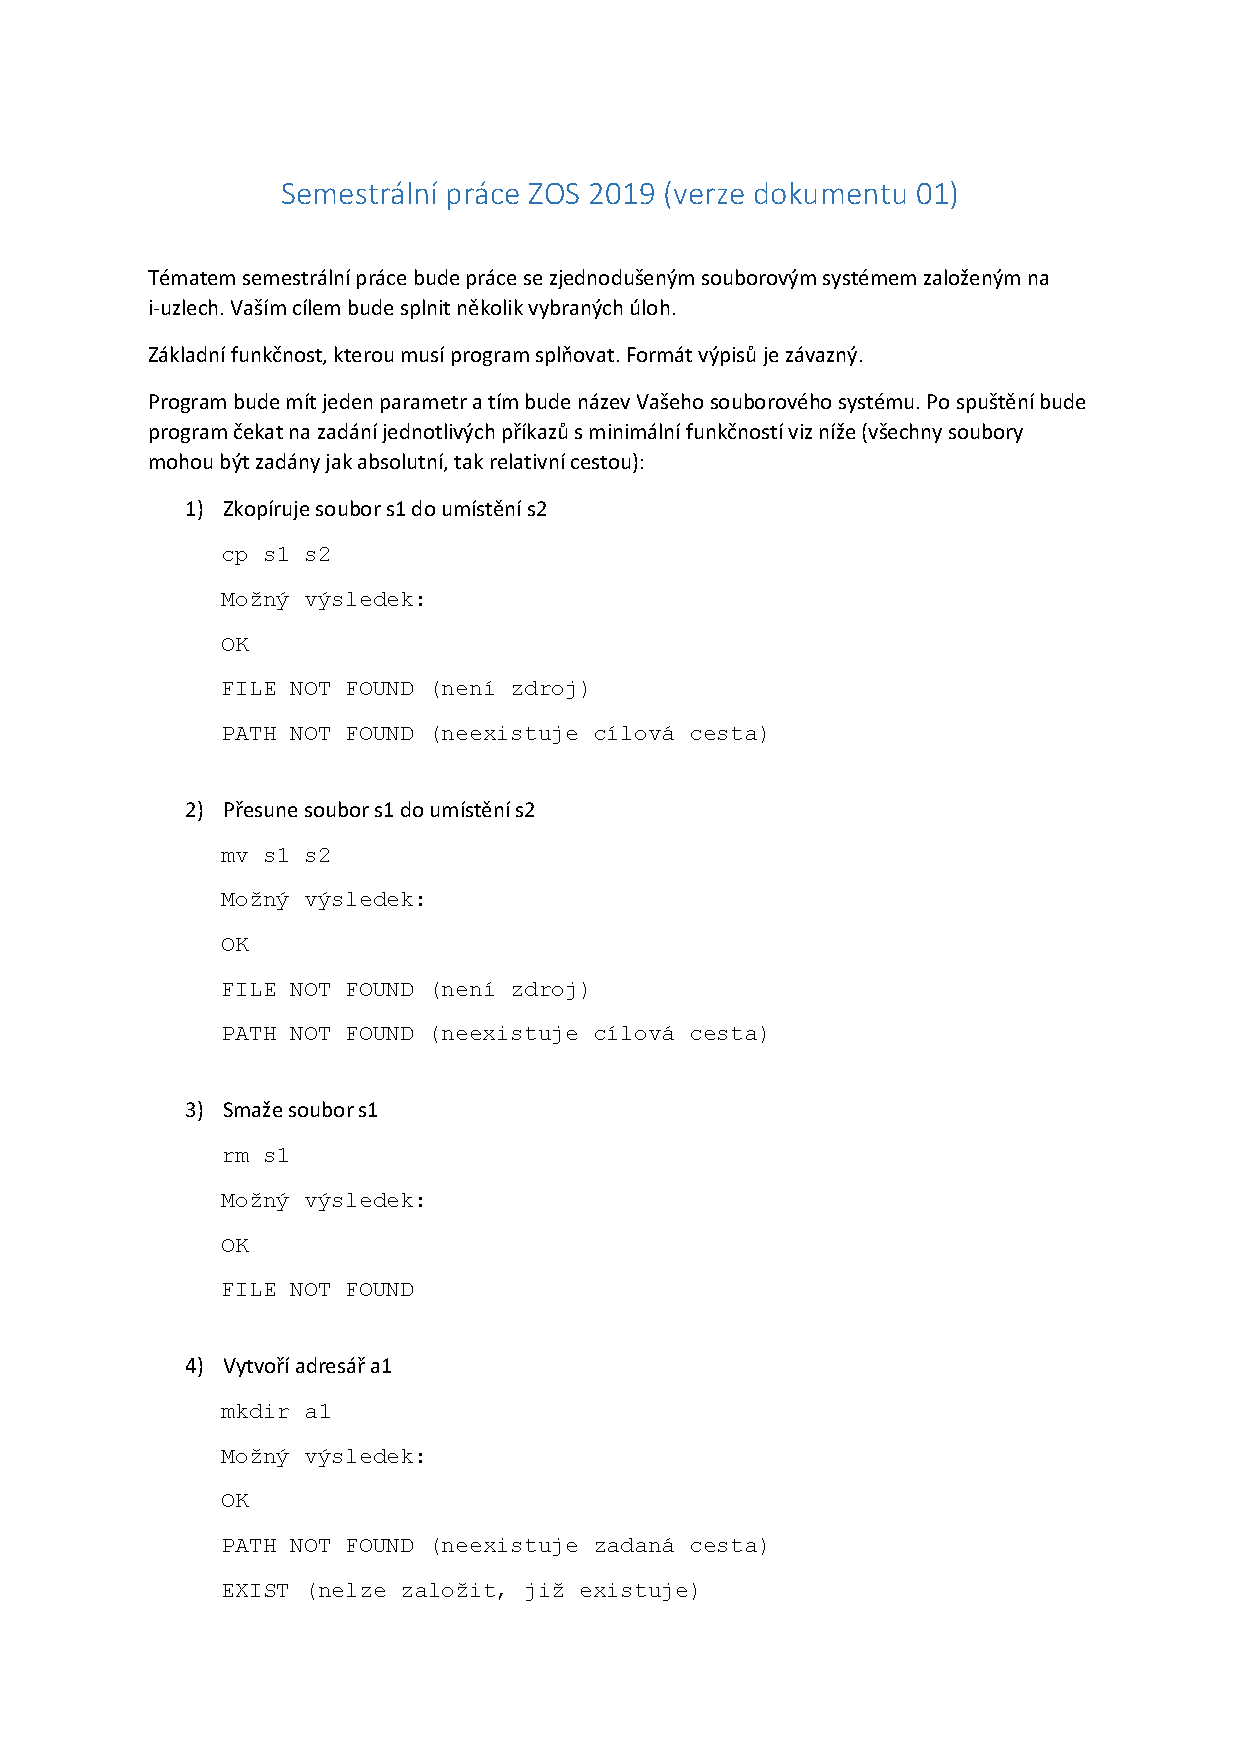
\includepdf[page=-]{zadani.pdf}

    \section{Analýza}
    \subsection{Datové struktury}
    Pro vytvoření souborového systému založeného na i-uzlech je potřeba několik základních struktur.
    Těmi jsou superblok, bitmapy pro obsazenost datových bloků a i-uzlů, i-uzel a samotný datový blok.


    \subsubsection{Superblok}
    Superblok je základní datová struktura, která je nezbytná pro fungování celého souborového systému.
    Uchovává základní informace o jeho struktuře, jako např. popis, počáteční adresy jeho částí, celkovou velikost, atd.

    \subsubsection{Bitmapa}
    Bitmapa je jednoduchá datová struktura, ve které je možné nastavit hodnotu biotu na konkrétní pozici na 0 nebo 1.
    Tato jednoduchá datová struktura se dá v souborovém systému použít ke značení, zda je daný i-uzel nebo datový blok volný k použití, nebo je obsazen.

    \subsubsection{I-uzel}
    I-uzel je datová struktura, která může být do velké míry chápána jako soubor.
    Na jeden soubor či složku totiž připadá právě jeden i-uzel.
    V této datové struktuře jsou obsaženy informace, pro možnost přečtení již zapsaného souboru.
    Jsou jimi například typ (složka/soubor), velikost zapsaných dat, počet naalokovaných datových bloků, a přímé/nepřímé odkazy na datové bloky.

    Přímé i nepřímé odkazy v i-uzlu odkazují na samotné datové bloky, kde jsou zapsaná požadovaná data.
    Každý typ odkazu k této problematice přistupuje mírně odlišně.

    Několik přímých odkazů je uloženo přímo v i-uzlu (zpravidla jednotky)
    V těchto odkazech jsou pak uloženy přímo odkazy na jednotlivé datové bloky s uloženými daty.

    Nepřímé odkazy už fungují mírně komplikovaněji.
    Odkaz, který je uložen v i-uzlu, neodkazuje na datový blok s daty, ale na datový blok s dalšími odkazy.
    Až tyto odkazy v datovém bloku nadále odkazují na jednotlivé datové bloky s daty.

    Nadále máme dvojité nepřímé odkazy, nicméně ty fungují velmi podobně.
    Jen s tím rozdílem, že se používá dvojitý odkaz (oproti jednoduchému).
    Odkaz v i-uzlu tedy odkazuje na datový blok s odkazy, kde každý odkaz odkazuje na další datový blok s odkazy, které už odkazují na jednotlivé datové bloky s daty.

    Takto bychom samozřejmě mohli pokračovat dále.
    Nicméně s každou násobností nepřímých odkazů velmi výrazně naroste maximální velikost souboru v souborovém systému.
    Z tohoto důvodu by třeba pětinásobné nepřímé odkazy nedávali smysl.
    Například souborový systém ext4 využívá nepřímé odkazy až do násobnosti tři.

    \begin{figure}
        \centering
        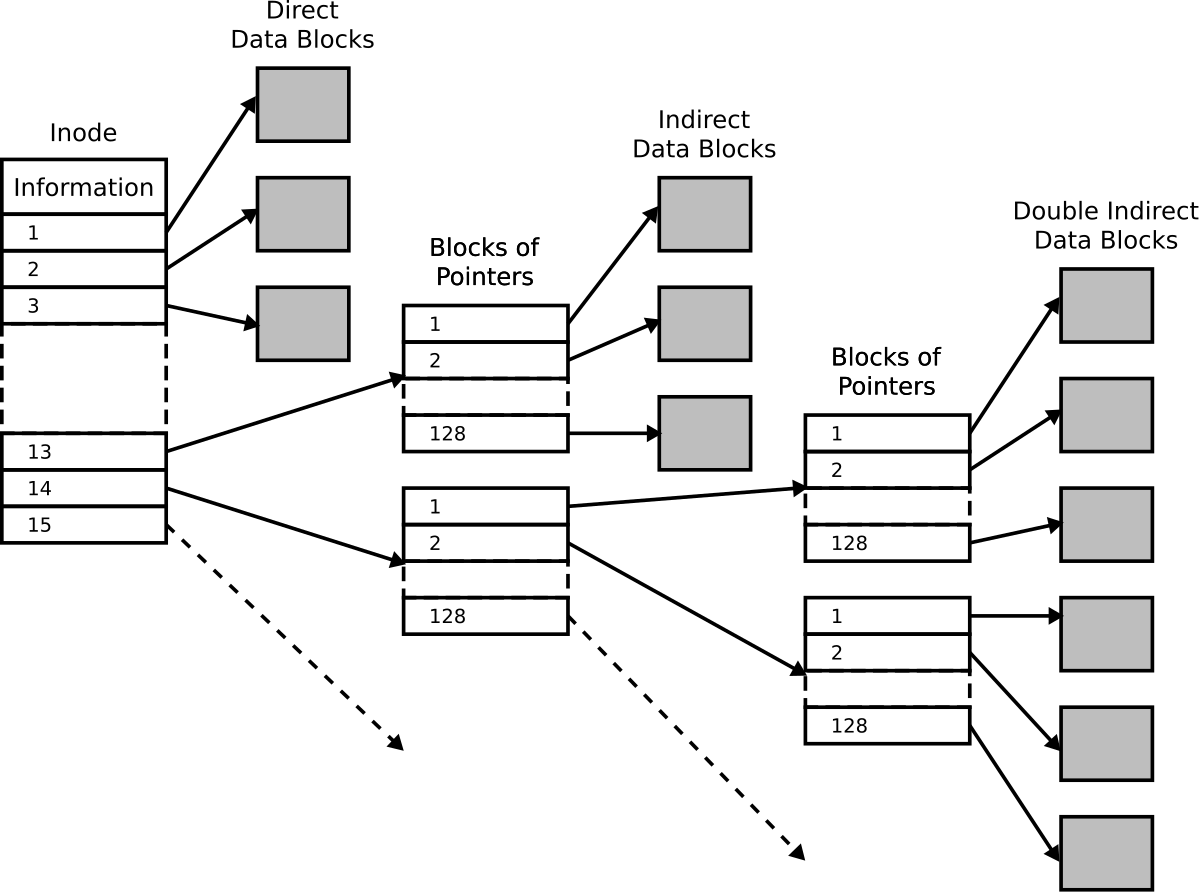
\includegraphics[width=\textwidth]{inode.png}
        \caption{Vizualizace struktury i-uzlu}
    \end{figure}

    \subsubsection{Datový blok}
    Datový blok představuje oblast v souborovém systému, kam je možné ukládat různá data.
    Můžou jimi být například přímo obsahy jednotlivých souborů, seznam souborů ve složce nebo odkazy na další datové bloky.

    \section{Implementace}
    Souborový systém byl především z časových důvodů implementován v jazyce Go.
    I přes toto rozhodnutí však nebylo zaznamenáno, že by samotná implementace jazyka jakkoliv snižovala výkon souborového systému.

    \subsection{Struktura souborového systému}
    Souborový potřebuje pro svou funkčnost pevnou strukturu jednotlivých jeho částí.
    Tyto části jsou pevně rozděleny již při formátování souborového systému a není možné je následně měnit.
    
    Souborový systém je na začátku rozdělen na 2 části. Na datovou část o velikosti 95\% celkové velikosti datového souboru, a na část, sloužící pro uložení i-uzlů, bitmap a superbloku, o velikosti 5\% celkové velikosti.

    Na začátku souborového systému je uložen superblok, následuje bitmapa pro označování obsazených datových bloků.
    A nakonec je zbylé místo využito na bitmapu použitých i-uzlů a samotné i-uzly.
    Velikost posledních dvou částí je vypočtena tak, aby se maximalizoval počet i-uzlů, a zároveň pro ně bylo možné vytvořit dostatečně velkou bitmapu.

    Při formátování souborového systému je celý datový soubor vynulován a ne jeho počátek je zapsán superblok s počátky adres výše uvedených částí.
    Díky tomu je formátování nenáročnou a rychlou operací.



    \subsection{Omezení souborového systému}
    Žádný souborový systém není plně bez omezení, i běžné souborové systémy mají řadu technických omezení.
    Jen na ně při běžném použití nenarazíme.
    U tohoto souborového systému tomu není jinak.

    Vytvořený souborový systém nemá žádnou ochranu proti jeho poškození.
    Ačkoliv poškození datové části pravděpodobně přežije, tak poškození ostatních jeho částí může vést ke ztrátě jednoho či více souborů.
    Poškození superbloku je pak nevratné a vede k poškození celého souborového systému.
    Kromě pokusu o ruční opravu zde není žádná jiná cesta jak souborový systém znovu obnovit.

    Maximální velikost souboru se pak odvíjí podle velikosti datového bloku.
    Tato hodnota se dá spočítat podle vzorce:\\$(pocet\_primych\_odkazu*velikost\_bloku+\frac{velikost\_bloku^2}{velikost\_odkazu}+\frac{velikost\_bloku^3}{velikost\_odkazu})$

    \subsection{API souborového systému}
    API, nebo-li aplikační rozhraní, souborového systému bylo implementováno tak, aby se co nejvíce podobalo práci se soubory, jak jí známe ze standardních souborových systémů (resp. operačního systému).
    Obsahuje tak operace jako například \texttt{Open}, \texttt{Read}, \texttt{Write}, \texttt{Rename} a další.
    Díky tomuto byla pak implementace příkazové řádky souborového systému triviální operací, jelikož už nebylo potřeba řešit žádné specifické problémy při práci s vytvořeným souborovým systémem.

    \subsection{Dostupné příkazy v příkazové řádce}
    Dostupné příkazy příkazové řádky jsou již velmi dobře zdokumentovány v přiloženém zadání.
    Z tohoto důvodu již nebudou opětovně zmíněny.
    Jediný příkaz, který je implementován nad rámec zadání, je \texttt{badrm}.
    Tento příkaz je implementován pouze pro ověření funkčnosti kontroly konzistence souborového systému.
    Jedná se o modifikaci příkazu \texttt{rm} s tím rozdílem, že neuvolní i-uzel zvoleného souboru.
    To má za následek to, že vznikne i-uzel, ke kterému nejde přistoupit, jelikož není v žádné složce v souborového systému.
    Tento příkaz tedy neslouží pro běžné smazání souboru, a je navržen tak, aby účelně poškodil souborový systém.


    \subsection{Použité knihovny}
    Vytvořený souborový systém používá pouze jednu knihovnu třetí strany, a tou je knihovna jménem \textit{ishell}.
    S pomocí této knihovny bylo možné velmi rychle a efektivně vytvořit prostředí příkazové řádky, které disponuje pokročilejšími funkcemi, jakými jsou například historie příkazů, vyhledávání v historii příkazů, automatické doplňování, atd.

    \subsection{Struktura implementace}
    Při programování souborového systému byl kladen důraz na oddělení základních částí implementace.
    Je tak oddělena práce se samotným úložištěm, i-uzly, tak i například alokace paměti pro i-uzly.
    Je tak teoreticky možné do budoucna zlepšit způsob alokace datových bloků tak, aby nebylo nutné alokovat pouze po jednom datovém bloku.
    Jelikož je alokace poměrně drahou operací, tak by tímto bylo teoreticky možné výrazným způsobem zvýšit výkon souborového systému.

    Celý souborový systém je implementován v modulu \texttt{vfs}, který už není dále členěn do modulů.
    Nicméně jak již bylo naznačeno výše, stále se zde dodržuje oddělení jednotlivých problematik souborového systému.

    Další modul přímo spjatý se souborovým systémem nese název \texttt{vfsapi}.
    Jedná se aplikační rozhraní určené pro použití třetí stranou.
    Je takto oddělené ve vlastním modulu, aby bylo zřejmé, co je určené pro vnější volání, a co už je funkce určená právě pro tvorbu API, a při nesprávném použití může způsobit nekonzistenci souborového systému.

    Posledním modulem je pak modul \texttt{shell}, který obsahuje implementaci jednotlivých příkazů příkazové řádky.
    Jednoduše řečeno se jedná o velmi tenkou vrstvu mezi příkazovým řádkem a API souborového systému.

    \section{Uživatelská příručka}
    \subsection{Překlad a sestavení projektu}
    Pro překlad a sestavení projektu je potřeba mít pouze nainstalovaný programovací jazyk go, a to minimálně ve verzi \texttt{1.13.6}.
    Následně už můžeme spustit kompilaci pouze pomocí \texttt{go build .}.
    Go automaticky stáhne všechny závislosti a provede překlad projektu.
    Pokud chceme projekt přímo spustit, tak je také možné použít příkaz \texttt{go run .}.
    Pro správnou funkčnost obou zmíněných příkazů je potřeba být v kořenovém adresáři projektu.

    \subsection{Ovládání}
    Po spuštění projektu je nadále možné pracovat se souborovým systémem jak je zvykem z prostředí GNU/Linux.
    Jsou implementovány všechny základní příkazy, jejichž podrobná dokumentace je dostupná v zadání semestrální práce.

    \section{Závěr}
    V rámci semestrální práce bylo nutné pochopit a implementovat základní principy souborových systémů.
    Ačkoliv se to zprvu jednalo o téměř nemožný úkol, tak se po řádném dekomponování problému ukázalo, že to není tak neproveditelné, jak by se mohlo zdát.

    Za největší problém implementace souborového systému bych označil to, že dlouho není vidět žádný použitelný výsledek.
    Nejdříve bylo nutné vůbec navrhnout strukturu souborového systému, následně implementovat bitmapy, i-uzly, alokátor datových bloků, a další komponenty
    Doba, od vytvoření projektu do zapsání prvního souboru, je tedy poměrně dlouhá.
    Reálné vytvoření souboru je dokonce tak pokročilá záležitost, že bylo implementováno v podstatě až při finalizaci celé semestrální práce.
    Jednalo se totiž v podstatě o pouhé propojení již připravených komponent, které bylo nutné předtím implementovat.
    Z těchto důvodů byly při vývoji aktivně používány jednotkové testy, které výrazně usnadnili detekci a opravování chyb v průběhu vývoje.
    Díky nim bylo možné ihned odhalit chybně implementovanou funkcionalitu, nebo rozbití již nějaké stávající.

    Co se týče samotného souborového systému, tak za jeho primární nedostatek bych označil jeho výkon a neodolnost vůči vnějším vlivům (chyba disku, výpadek proudu, náhlé odpojené disku, \dots).
    Ačkoliv nakopírovat soubor o velikosti 40MB trvá zhruba jednu sekundu, tak nakopírování souboru o velikosti 1GB je záležitostí na několik minut.
    Tento jev přisuzuji právě pomalému alokátoru, který hledá volné datové bloky lineárně a vždy od začátku.
    Ke zrychlení by mohlo dojít například, kdyby se nealokovalo pouze po jednom datovém bloku, ale například po čtyřech.

    Souborový systém má samozřejmě i spoustu dalších nedostatků, nicméně pro jejich vyřešení už by se nemohlo jednat o semestrální práci, ale spíše o dlouhodobý několikaletý projekt.

    I přes zmíněné nedostatky jsem však s výslednou prací spokojen a podle zadání je splněna.

    \newpage
    \listoffigures
    


\end{document}
